\documentclass{beamer}
\usetheme{Warsaw}
\usepackage{graphicx}
\usepackage{tikz}
\usepackage{colortbl}
\setbeamertemplate{footline}[frame number]

\title{Ensemble Clustering}
\subtitle{Seminar im Fachgebiet Wissensverarbeitung}
\author{Malek Alsalamat}
\institute{Universität Kassel}

\begin{document}
	
\begin{frame}
	\titlepage
\end{frame}

\begin{frame}{Inhalt der Präsentation}
	In der Präsentation werden wir folgendes behandeln: 
	\begin{enumerate}
		\item Was ist Clustering
		\item K-Means 
		\item Ensemble Clustering und das Ensemble Problem
		\item Zielfunktion
		\item Effiziente consensus Funktion
		\item Cluster-based Similarity Partitioning Algorithm
		\item Anwendungen
	\end{enumerate}
\end{frame}

\begin{frame}{Was ist Clustering}
	\begin{block}{Definition von Clustering}
		\textbf{Clustering} ist die Methode im maschinellen Lernen und genauer gesagt “im unüberwachten Lernen”, Datenpunkte in Gruppen (Clusters) ohne vorhandenes Wissen zu ordnen.  Um das zu schaffen, wird die Ähnlichkeit zwischen die Daten berechnet.
	\end{block}
\only<1>{Ziel von Clustering: 
	\begin{itemize}
		\item Ähnliche Datenpunkte (Objekte) sollen im selben Cluster sein. 
		\item Datenpunkte im verschiedenen Cluster soll möglichst unähnlich sein.   
\end{itemize}}
\only<2>{\begin{block}{Beispiel.1}
		Cluster unterschiedlicher Größe, Form und Dichte bzw. hierarchische Cluster
		\begin{figure}[h]
			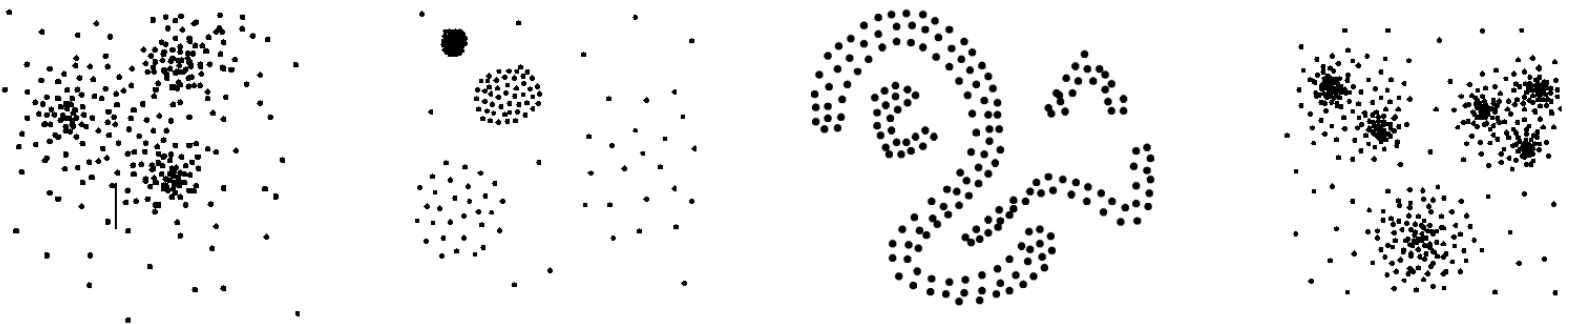
\includegraphics[width=\linewidth]{pic1}
		\end{figure}
\end{block}}
\end{frame}

\begin{frame}{K-Means als Beispiel für partitionierende Verfahren}
	\only<1>{Im partitionierenden Verfahren wird ein Clustering mit k Cluster mit minimalen Kosten gesucht. Und bei K-Means wie der Name bereits sagt, sucht das Algorithmus für jeden Cluster einen zentralen Punkt, bei dem die Varianz zu allen umliegenden Punkten möglichst gering ist.
		Das Ganze passiert in einem iterativen Verfahren wie folgendes:}
	\begin{enumerate}
		\item Initialisierung: Zufällige Auswahl von K Zentren. 
		\item Zuweisung aller Datenpunkten zum nächstliegenden Zentrum, gemessen an einer Distanzmetrik. Distanzmetrik berechnet hier die Ähnlichkeit. 
		\item Verschieben der Zentren in den Mittelpunkt aller zugeteilten Datenpunkte.
		\item Gehe zu 2), außer ein Abbruchkriterium ist erreicht. Der Abbruchkriterium ist, wenn die Zentren sich nicht mehr ändern.    
	\end{enumerate}

\end{frame}

\begin{frame}{Ensemble Clustering}
	\begin{block}{Definition}
		Im Zusammenhang mit maschinellem Lernen ist Ensemble im Allgemein definiert
		als ein maschinelles Lernsystem, das mit einer Reihe von parallel arbeitenden
		einzelnen Modellen konstruiert wird. Und die Ergebnisse von diesen Modellen
		werden mit einer Entscheidungsstrategie kombiniert, um einzige Lösung
		für das gegebenen Problem zu liefern.
	\end{block}
	\only<2>{Die Gründe für die Anwendung der Ensemble Methode auf Clustering Probleme sind:
	\begin{enumerate}
		\item Es gibt kein vorhandenes Wissen über die zugrundeliegende Struktur
		\item Es gibt keinen einzelnen Clustering-Algorithmus, der für verschiedene Probleme konsistent gute Leistungen erbringen kann.
\end{enumerate}}
\end{frame}

\begin{frame}{Das Ensemble Problem}
	\begin{block}{Gegeben}
		Mehrere Clusterings aus verschiedenen Algorithmen von derselben Datenmenge.
	\end{block}
	\begin{block}{Gesucht}
		Ein kombiniertes Clustering, welches so viele Informationen wie möglich mit den gegebenen Clusterings teilt. 
	\end{block}
	\textbf{Notation}: Sei $X$ = $\{x_1, x_2, \ldots, x_n\}$ eine Menge von Objekten (Datenpunkte). Eine Partitionierung dieser $n$ Objekten in $k$ Clusters kann als eine Menge von k Mengen von Objekten $\{C_{l} \mid l = 1, \ldots, k\}$ oder als ein Label Vektor $\lambda \in {N}^{n}$ dargestellt werden. Ein Clusterer $\Phi$ ist eine Funktion, welche einen Label Vektor bei gegebene Objekten liefert. Eine Mengen von $r$ Clusterings (Labelings) $\lambda^{(1, \dots, r)}$ kann zu einem Clustering anhand einer Consensus Funktion kombiniert werden.
\end{frame}


\begin{frame}{Das Ensemble Problem}
	Sei $X$ = $\{x_1, x_2, \ldots, x_7\}$ eine Menge von Objekte und 3 Clusters $\{C_{l}, C_{2}, C_{3}\}$ und die Clustering $\lambda^{(1, \dots, r)}$ wie in der Tabelle gezeigt.
	\only<1>{\begin{center}
			\begin{tabular}{  l| c c c c}
				\quad & $\lambda^{(1)}$ & $\lambda^{(2)}$ & $\lambda^{(3)}$ & $\lambda^{(4)}$  \\ \hline 
				$x_1$ & 1 & 2 & 1 & 1  \\
				$x_2$ & 1 & 2 & 1 & 2  \\
				$x_3$ & 1 & 2 & 2 & ?  \\
				$x_4$ & 2 & 3 & 2 & 1  \\
				$x_5$ & 2 & 3 & 3 & 2  \\
				$x_6$ & 3 & 1 & 3 & ?  \\ 
				$x_7$ & 3 & 1 & 3 & ?  \\
			\end{tabular}
	\end{center}} 
	
	\only<2>{\begin{center}
			\begin{tabular}{  l| c c c c}
				\quad & $\lambda^{(1)}$ & $\lambda^{(2)}$ & $\lambda^{(3)}$ & $\lambda^{(4)}$  \\ \hline 
				$x_1$ & \cellcolor{green}1 & 2 & 1 & 1  \\
				$x_2$ & \cellcolor{green}1 & 2 & 1 & 2  \\
				$x_3$ & \cellcolor{green}1 & 2 & 2 & ?  \\
				$x_4$ & \cellcolor{red}2 & 3 & 2 & 1  \\
				$x_5$ & \cellcolor{red}2 & 3 & 3 & 2  \\
				$x_6$ & \cellcolor{blue}3 & 1 & 3 & ?  \\ 
				$x_7$ & \cellcolor{blue}3 & 1 & 3 & ?  \\
			\end{tabular}
	\end{center}}

	\only<3>{\begin{center}
			\begin{tabular}{  l| c c c c}
				\quad & $\lambda^{(1)}$ & $\lambda^{(2)}$ & $\lambda^{(3)}$ & $\lambda^{(4)}$  \\ \hline 
				$x_1$ & 1 & \cellcolor{red}2 & 1 & 1  \\
				$x_2$ & 1 & \cellcolor{red}2 & 1 & 2  \\
				$x_3$ & 1 & \cellcolor{red}2 & 2 & ?  \\
				$x_4$ & 2 & \cellcolor{blue}3 & 2 & 1  \\
				$x_5$ & 2 & \cellcolor{blue}3 & 3 & 2  \\
				$x_6$ & 3 & \cellcolor{green}1 & 3 & ?  \\ 
				$x_7$ & 3 & \cellcolor{green}1 & 3 & ?  \\
			\end{tabular}
	\end{center}}

	\only<4>{\begin{center}
			\begin{tabular}{  l| c c c c}
				\quad & $\lambda^{(1)}$ & $\lambda^{(2)}$ & $\lambda^{(3)}$ & $\lambda^{(4)}$  \\ \hline 
				$x_1$ & 1 & 2 & \cellcolor{green}1 & 1  \\
				$x_2$ & 1 & 2 & \cellcolor{green}1 & 2  \\
				$x_3$ & 1 & 2 & \cellcolor{red}2 & ?  \\
				$x_4$ & 2 & 3 & \cellcolor{red}2 & 1  \\
				$x_5$ & 2 & 3 & \cellcolor{blue}3 & 2  \\
				$x_6$ & 3 & 1 & \cellcolor{blue}3 & ?  \\ 
				$x_7$ & 3 & 1 & \cellcolor{blue}3 & ?  \\
			\end{tabular}
	\end{center}}

	\only<5>{\begin{center}
			\begin{tabular}{  l| c c c c}
				\quad & $\lambda^{(1)}$ & $\lambda^{(2)}$ & $\lambda^{(3)}$ & $\lambda^{(4)}$  \\ \hline 
				$x_1$ & 1 & 2 & 1 & 1  \\
				$x_2$ & 1 & 2 & 1 & 2  \\
				$x_3$ & 1 & 2 & 2 & ?  \\
				$x_4$ & 2 & 3 & 2 & 1  \\
				$x_5$ & 2 & 3 & 3 & 2  \\
				$x_6$ & 3 & 1 & 3 & ?  \\ 
				$x_7$ & 3 & 1 & 3 & ?  \\
			\end{tabular}
	\end{center}
	Gesucht ist jetzt ein kombiniertes Clustering, welches so viele Informationen wie möglich mit den vier gegebenen Clusterings teilt. Intuitiv, ein gutes kombiniertes Clustering in diesem Fall ist  $\lambda^{(1)}$ oder auch $\lambda^{(2)}$.}
\end{frame}

\begin{frame}{Zielfunktion für Ensemble Clustering}
	\begin{block}{Definition}
		Gegeben nun $r$ Gruppierungen mit $\lambda^{(i)}$ ist die $i$-te Gruppierung, welche $k^{i}$ Clusters hat. Eine $consensus$ Funktion ist wie folgt definiert $\Gamma:\mathbb{N}^{n \times r} \rightarrow \mathbb{N}^{n}$.
		\begin{equation} 
			\centerline{ $\Gamma$ : $\{\lambda^{i} \mid i \in {1, \ldots, r}\} \rightarrow \lambda$.}
		\end{equation}
	\end{block}
	
Eine sinnvolle Ziel für die $consensus$ Funktion ist, ein Clustering zu suchen, welches die meisten Informationen mit den ursprünglichen \textbf{Clusterings} teilt.
\end{frame}

\begin{frame}{Zielfunktion für Ensemble Clustering}
	Sei $n_{h}^{(a)}$ die Anzahl von Objekten in Cluster $C_{h}$ anhand das Clustering $\lambda^{(a)}$ und $n_{l}^{(b)}$ die Anzahl von Objekten in Cluster $C_{l}$ anhand das Clustering $\lambda^{(b)}$. Sei $n_{h,l}$ die Anzahl der gemeinsamen Objekten zwischen Cluster $h$ anhand $\lambda^{(a)}$ und Cluster $l$ anhand $\lambda^{(b)}$. Dann ist:
	\begin{equation}
		\centerline{$\phi^{(NMI)}(\lambda^{(a)}, \lambda^{(b)}) = \frac{\sum_{h=1}^{k^{(a)}} \sum_{l=1}^{k^{(b)}}n_{h,l} \cdot \log \biggl(\frac{n \cdot n_{h,l}}{n_{h}^{(a)} \cdot n_{l}^{(b)}} \biggr) }{\sqrt{\biggl(\sum_{h=1}^{k^{(a)}} n_{h}^{(a)} \log \frac{n_{h}^{(a)}}{n} \biggr)
					\biggl(\sum_{l=1}^{k^{(b)}} n_{l}^{(b)} \cdot \log \frac{n_{l}^{(b)}}{n} \biggr)}}.$}
	\end{equation}
\end{frame}

\begin{frame}{Zielfunktion für Ensemble Clustering}
	Von Gleichung $(2)$ wird einen Maß zwischen einer Menge $\Lambda$ und einem einzelnen Clustering $\hat{\lambda}$  als die durchschnittliche normalisierte gegenseitige Information definiert (ANMI): 
	\begin{equation} 
		\centerline{$\phi^{(ANMI)}(\Lambda, \hat{\lambda}) = \frac{1}{r} \sum_{q=1}^{r} \phi^{(NMI)}(\hat{\lambda}, \lambda^{(q)}).$}
	\end{equation}
	\only<2>{Das optimale kombinierte Clustering $\lambda^{(k-opt)}$ ist das Clustering mit der maximalen durchschnittlichen gegenseitigen Information, wobei $k$ ist die Anzahl von $consensus$ Clusters. In anderen Worten, $\phi^{(ANMI)}$ ist unsere Zielfunktion und $\lambda^{(k-opt)}$ ist:
		\begin{equation} 
			\centerline{$\lambda^{(k-opt)} = \underset{\hat{\lambda}}{\arg\max} \sum_{q=1}^{r} \phi^{(NMI)}(\hat{\lambda}, \lambda^{(q)}),$}
		\end{equation}
		wobei $\hat{\lambda}$ durch alle mögliche $k-Partitionierungen$ läuft.}
	
\end{frame}

\begin{frame}{Effiziente consensus Funktion}
	
	\begin{figure}[h]
		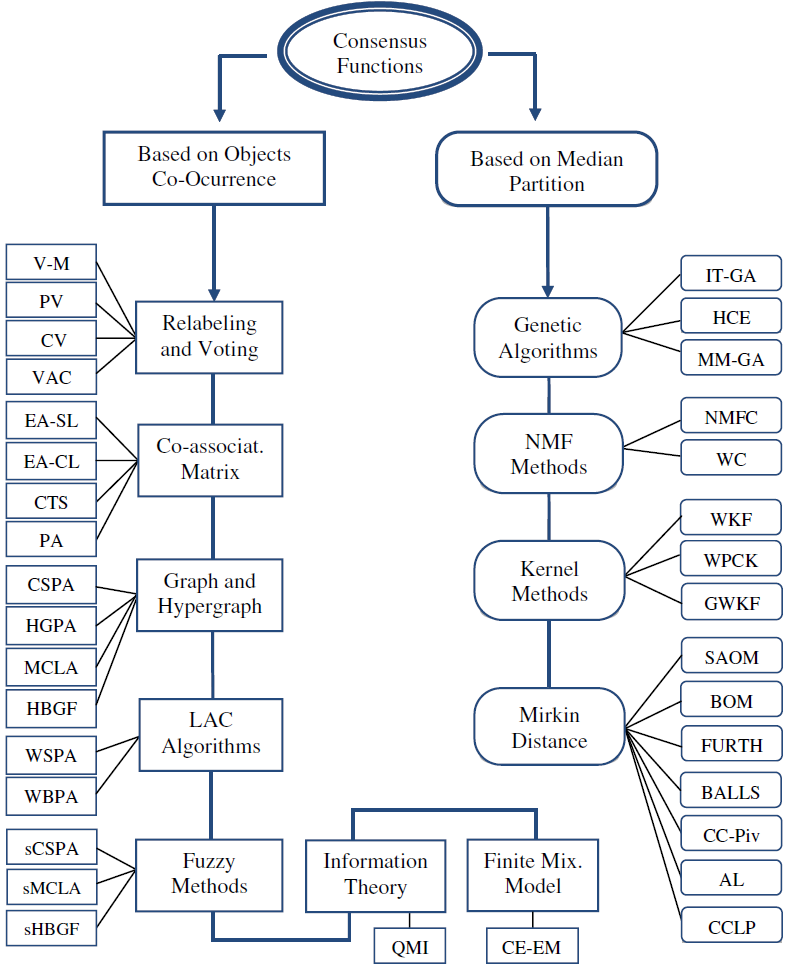
\includegraphics[width=0.7\linewidth, height=0.7\textheight]{pic3}
	\end{figure}
	
\end{frame}

\begin{frame}{Graph and hypergraph based methods}
	\only<1>{\begin{block}{Cluster-based Similarity Partitioning Algorithm (CSPA)}
			 Hier wird aus dem Hypergraph eine $n \times n$ Ähnlichkeitsmatrix (die Co-Assoziationsmatrix) konstruiert. Dies kann als eine Adjazenzmatrix eines zusammenhängenden Graphen angesehen werden, wobei die Knoten die Elemente der Datenmenge $X$ sind und die kanten zwischen zwei Objekten ein zugeordnetes Gewicht hat. Das Gewicht entspricht, wie oft sich die Objekte im selben Cluster befinden. Danach wird das Graph-Partitionierungsalgorithmus MEITS verwendet, um die $consensus$ Partitionierung zu erhalten.
	\end{block}}

	\only<2>{\begin{block}{HyperGraphs Partitioning Algorithm (HGPA)}
			Hier wird den Hypergraphen direkt partitioniert, indem die minimale Anzahl  von Hyperkanten eliminiert wird. Außerdem wird es davon ausgegangen, dass alle Hyperkanten das gleiche Gewicht haben. Und es wird nach der kleinstmöglichen Anzahl von Hyperkanten gesucht, die den Hypergraphen in $k$ zusammenhängende Komponenten von
			annähernd gleicher Dimension unterteilen. Für die Implementierung dieser Methode wird die Hypergraphs-Partitionierungspaket $HMETIS$ verwendet.
	\end{block}}

	\only<3>{\begin{block}{Hybrid Bipartite Graph Formulation (HBGF)}
			In diesem letzten Algorithmus werden die Clusters und Objekten zusammen in derselben Graph modelliert. Bei dieser Methode wird der bipartite-Graph so gebildet, dass es keine Kanten zwischen Knoten gibt, falls sie beide entweder Objekte oder Clusters sind. Also es gibt nur Kanten zwischen zwei Knoten, falls ein Knoten einem Cluster repräsentiert und der Zweite einem Objekt, der zu diesem Cluster gehört, repräsentiert. Die $consensus$ Partitionierung wird unter der Verwendung von METIS oder $Spectral-Clustering$ erhalten.
	\end{block}}
\end{frame}

\begin{frame}{Darstellung von Gruppen von Clusterings als Hypergraph}
	Für jeden Label Vektor $(Clustering)$ $\lambda^{(q)} \in \mathbb{N}^{n}$ konstruieren wir die binäre Zugehörigkeitsindikatormatrix  $H^{(q)} \in \mathbb{N}^{n \times k^{(q)}}$, wobei jeder Cluster als Hyperkante $(Spalte)$ dargestellt wird (Siehe Abb.2). Alle Einträge einer Zeile in der binären Zugehörigkeitsindikatormatrix $H^{(q)}$ werden zu 1 addiert, falls die Zeile mit einem Objekt, welches sein Cluster bekannt ist, übereinstimmt. und Zeilen für Objekte mit unbekanntem Cluster sind mit Null ausgefüllt.\\
	Die Blockmatrix $H = (H^{(1)} \ldots H^{(r)})$ definiert die Adjazenzmatrix eines Hypergraphen mit $n$ Knoten und $\sum_{q=1}^{r} k^{(q)}$ Hyperkanten. Jeder Spaltenvektor $\boldsymbol{h_{a}}$ spezifiziert eine Hyperkante $h_{a}$, wobei 1 anzeigt, dass der Knoten mit der entsprechenden Zeile zu der Hyperkante gehört und 0 gibt an, dass dies nicht der Fall ist. Somit haben wir jeder Cluster zu einem Hyperkante und die Menge von Clusterings zu einem Hypergraph abgebildet.
\end{frame}

\begin{frame}{Darstellung von Gruppen von Clusterings als Hypergraph}
	Beispiel für die Umwandlung von Clusterings zu einem Hypergraph:
	\begin{figure}[h]
		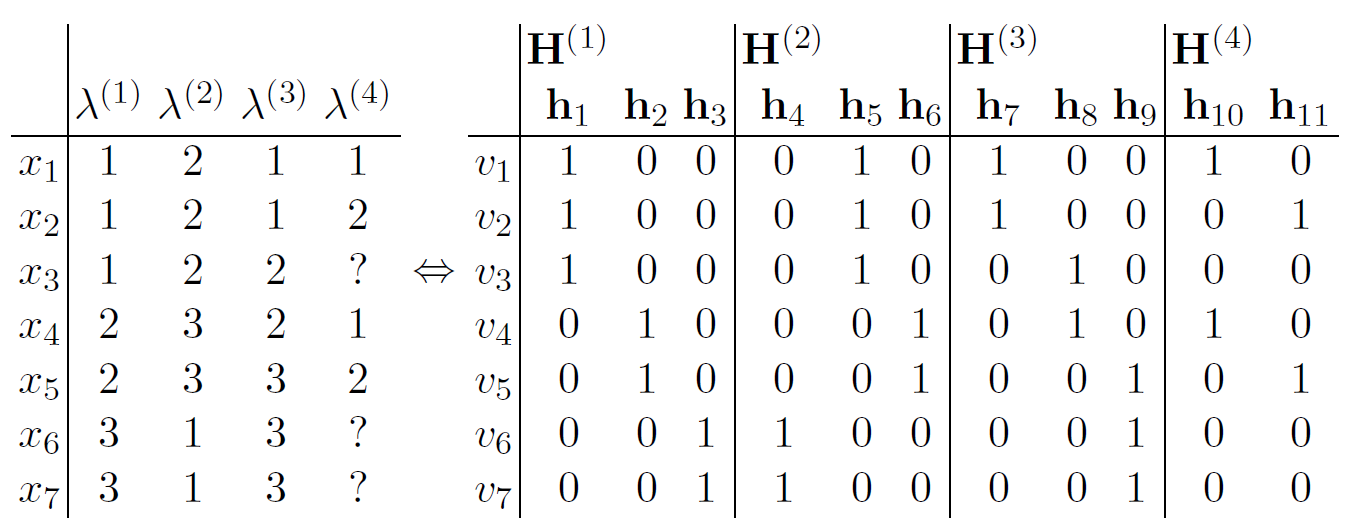
\includegraphics[width=0.9\linewidth]{pic4}
	\end{figure}
\end{frame}

\begin{frame}{Cluster-based Similarity Partitioning Algorithm}
	\begin{enumerate}
		\item Der eingangsbezogene Durchschnitt von $r$ solchen Matrizen, die die $r$ Gruppen darstellen, ergibt eine Gesamtähnlichkeitsmatrix S mit einer feineren Auflösung. Einträge von S bezeichnen den Anteil der Gruppierungen, in denen sich zwei Objekte im selben Cluster befinden,
		und können mit einer einzigen dünnbesetzten Matrixmultiplikation $(sparse- matrix)$ berechnet werden S = $\frac{1}{r} H H^{T}$.
		\only<2>{\item Nun können wir die Ähnlichkeitsmatrix verwenden, um die Objekte mit einem beliebigen sinnvollen
			Clustering-Algorithmus auf der Basis von Ähnlichkeit zu $reclustern$. In unserem Fall entscheiden wir uns für eine Partitionierung des induzierten Ähnlichkeitsgraphen (Knote = Objekt, Kantengewicht = Ähnlichkeit) mit METIS}
	\end{enumerate}
	
\end{frame}

\begin{frame}{Cluster-based Similarity Partitioning Algorithm}
	\only<1>{ Berechnung von $S$ für das Ensemble Problem:
		\begin{center}
			$r \cdot S$ = \quad
			\begin{tabular}{  l| c c c c c c c}
				\quad & $x_1$ & $x_2$ & $x_3$ & $x_4$ & $x_5$ & $x_6$ & $x_7$ \\ \hline 
				$x_1$ & 4 & 3 & 2 & 1 & 0 & 0 & 0 \\
				$x_2$ & 3 & 4 & 2 & 0 & 1 & 0 & 0 \\
				$x_3$ & 2 & 2 & 3 & 1 & 0 & 0 & 0 \\
				$x_4$ & 1 & 0 & 1 & 4 & 2 & 0 & 0 \\
				$x_5$ & 0 & 1 & 2 & 4 & 1 & 1 & 1 \\
				$x_6$ & 0 & 0 & 0 & 0 & 1 & 3 & 3 \\ 
				$x_7$ & 0 & 0 & 0 & 0 & 1 & 3 & 3 \\
			\end{tabular}
	\end{center}}
	\only<2>{Veranschaulichung von (CSPA) für das in Abb.2 angegebene Cluster-Ensemble-Beispielproblem. Jedes Clustering besitzt eine
		Ähnlichkeitsmatrix. Die Matrixeinträge werden durch Dunkelheit proportional zur Ähnlichkeit dargestellt.
		Ihr Durchschnitt wird dann verwendet, um die Objekte neu zu clustern und einen Konsens zu erhalten. 
		\begin{figure}[h]
			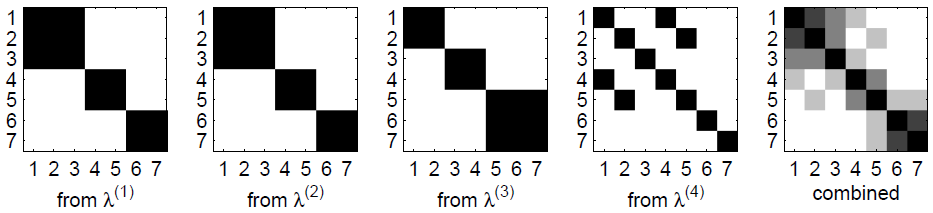
\includegraphics[width=\linewidth]{pic5}
		\end{figure}}
\end{frame}

\begin{frame}{Mehrstufige Graphenbisektion}
	Ein mehrstufiger Graphbisektionsalgorithmus funktioniert wie folgt: betrachte einen gewichteten Graphen $G_0 = (V_0, E_0)$ mit Gewichten sowohl aus Knoten als auch auf Kanten. Dieser Algorithmus besteht aus den folgenden drei Phasen:
	\begin{enumerate}
		\item Vergröberungsphase $Coarsening$: Der Graph $G_0$ wird in ein Folge von kleineren Graphen $G_1, G_2, \ldots, G_m$ umgewandelt, so dass $\lvert V_0 \lvert > \lvert V_1 \lvert > \ldots > \lvert V_m \lvert.$
		\only<2,3>{\item Partitionierungsphase: Eine 2-fache-Partition $P_m$ des Graphen $G_m = (V_m, E_m)$ wird berechnet, die $V_m$ in zwei Teile unterteilt, die jeweils die Hälfte der Knoten von $G_0$ enthält.}
		\only<3>{\item Entgröberungsphase $Uncoarsening$: Die Partition $P_m$ von $G_m$ wird auf $G_0$ zurückprojiziert, indem man durch die Zwischenpartitionen $P_{m-1}, P_{m-2}, \ldots, P_1, P_0$ geht.}
	\end{enumerate}
\end{frame}

\begin{frame}{Mehrstufige Graphenbisektion}
	\begin{figure}[h]
		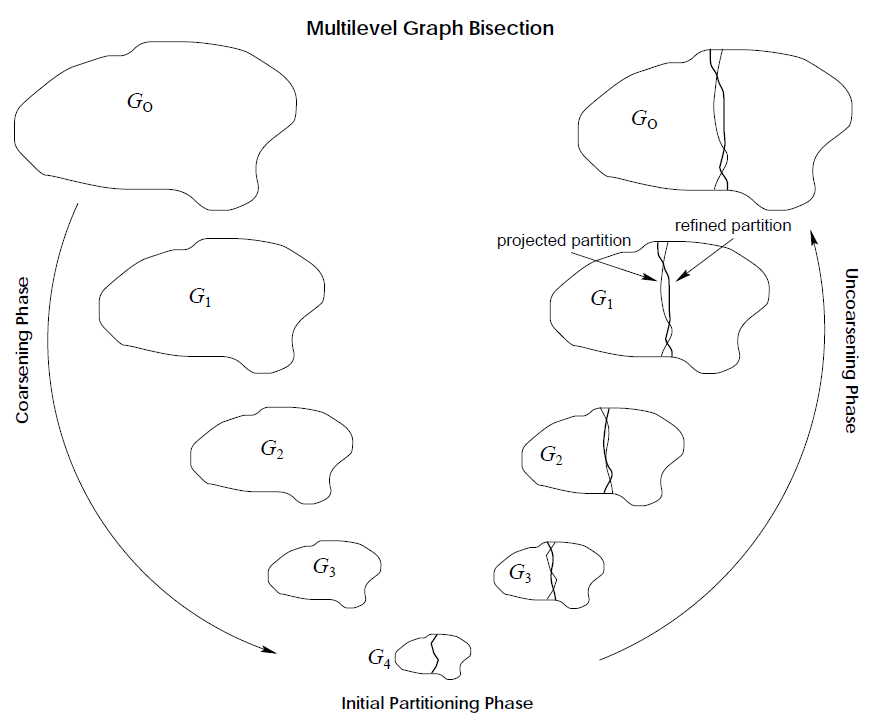
\includegraphics[width=0.7\linewidth, height=0.7\textheight]{pic6}
	\end{figure}
\end{frame}

\begin{frame}{Vergröberungsphase $(Coarsening)$}
	\only<1>{\begin{figure}[h]
			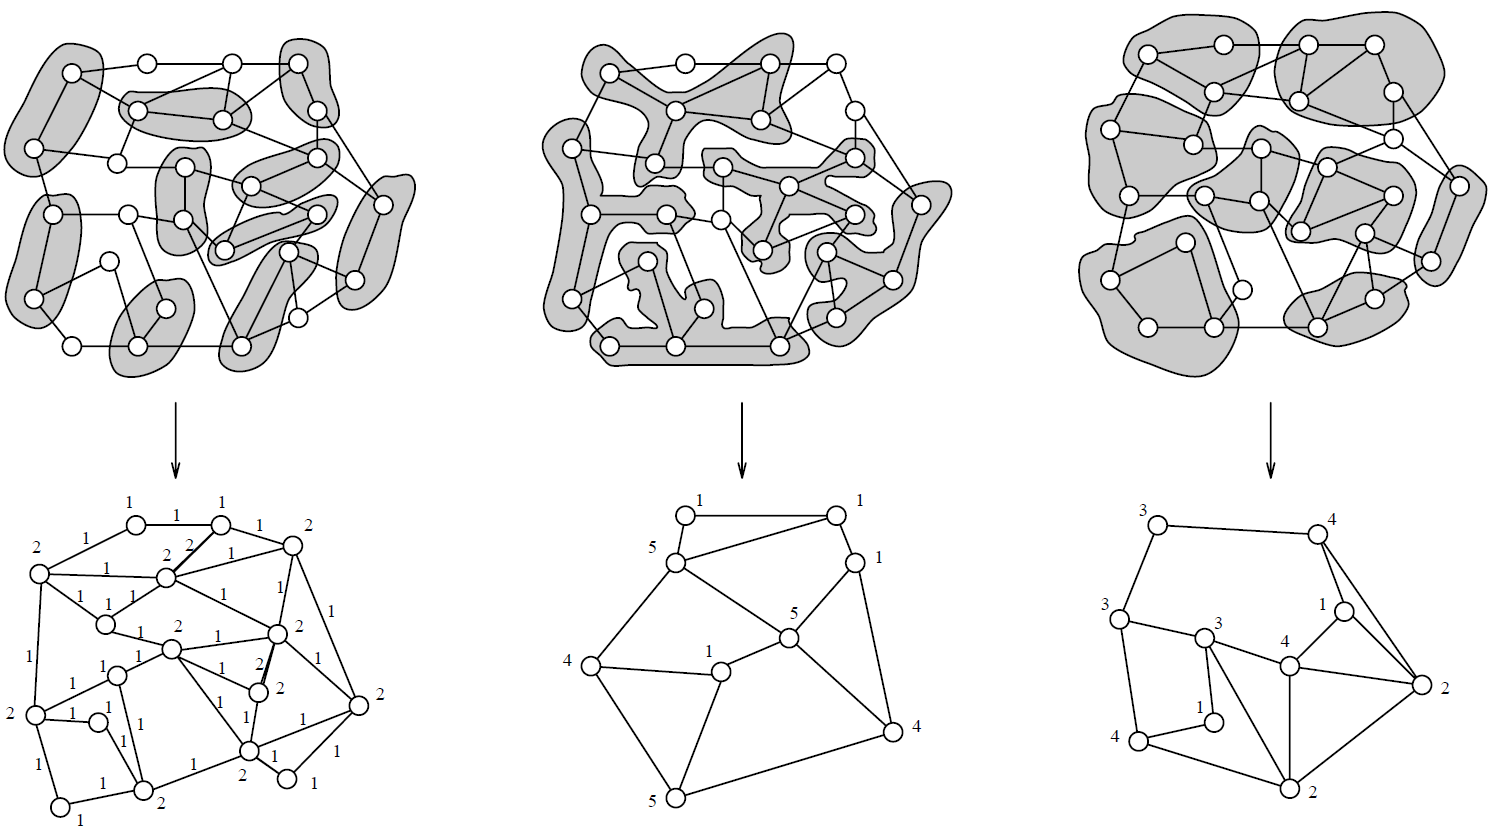
\includegraphics[width=\linewidth]{pic7}
	\end{figure}}
	\only<2>{\begin{block}{Random matching (RM)}
			 Ein maximales Matching kann mit einen randomisierten Algorithmus generiert werden. Die Knoten sind dann in  zufälliger Reihenfolge besucht. Wenn ein Knoten $u$ noch nicht ausgewählt wurde, dann wählen wir einen seiner nicht ausgewählter Nachbarknoten aus. Wenn es solcher Knoten $v$ existiert, wird die Kante $(u, v)$ zum Matching gefügt und markieren wir die Knoten $u$ und $v$ als besucht. Wenn es keinen solchen Konten $v$ gibt, dann bleibt $u$  wie es ist in der $RM$. Die Komplexität von diesem Algorithmus liegt in $O(\lvert E \lvert)$.
		\end{block}}
\end{frame}

\begin{frame}{Partitionierungsphase}
	Ziel von der Partitionierungsphase ist den Graphen in zwei Teile zu schneiden so, dass jeder Teil ungefähr die Hälfte des Knotengewichts des ursprünglichen Graphen enthält.
	Eine Partition von $G_m$ kann mit verschiedenen Algorithmen erhalten werden, wie z.B: 
	\begin{enumerate}
		\only<1,2,3>{\item spektrale Bisektion $SB$}
		\only<2,3>{\item geometrische Bisektion (wenn Koordinaten verfügbar sind)}
		\only<3>{\item kombinatorische Methoden}
	\end{enumerate}
\end{frame}

\begin{frame}{Graph growing partitioning algorithm (GGP)}
	\begin{block}{GGP}
		Eine einfache Methode zur Bisektion des Graphen und sie funktioniert wir folgt:\\
		Man startet bei einem beliebigen Knoten und bildet eine Region um ihn herum, bis die Hälfte der Knoten oder die Hälfte des gesamten Knotengewichtes einbezogen ist. Die Qualität des $GGP$ ist abhängig von der Wahl eines Knotens, von dem aus das Wachstum des Graphen beginnt, und verschiedene Startknoten ergeben unterschiedliche Kantenschnitte.  
		Um dieses Problem teilweise zu lösen, wählen wir zufällig 10 Eckpunkte
		und lassen 10 verschiedene Regionen wachsen. Der Versuch mit dem kleineren Kantenschnitt wird als
		die Partition ausgewählt.
	\end{block}
\end{frame}


\begin{frame}{Entgröberungsphase $(Uncoarsening)$}
	Inhalt...
\end{frame}

\begin{frame}{Anwendungen}
	\begin{block}{Segmentierungskombination}
		Der Random-Walker-Algorithmus wird für einen
		ungerichteten Graphen $G = (V, E, w)$ formuliert, in dem jedes Pixel
		$p_i$ einen entsprechenden Knoten $v_i \in V$ hat. Jede Kante $e_{ij} \in E$  hat ein Gewicht $w_{ij}$, das die Ähnlichkeit zwischen den benachbarten Pixeln $v_i$ und $v_j$  (in 4-Nachbarschaft). In diesem $Framework$ wird der Anzahl der Regionen in einem Bild als $K$ bezeichnet. Der tatsächliche Anzahl ist eigentlich nicht bekannt. Bei der Berechnung einer Reihe von Kombinationssegmentierungen
		mit $K \in [K_{min}, K_{max}]$ Seed-Regionen, brauchen wir ein Verfahren um
		die optimale Region auszuwählen. In[7] wird die optimale Segmentationskombination $S^{kopt}$ so ausgewählt, dass es die eine mit maximale durchschnittliche gegenseitige Information zwischen alle Segmentastionen $S_q$ in $\Lambda$, wobei $\Lambda  = \{S_1, \ldots ,S_N\}$ ist. Die optimale $S^{kopt}$ wird nach der Gleichung $(5)$ berechnet, wobei $\hat{\lambda}$ bedeckt all mögliche  $K \in [K_{min}, K_{max}]$  Segmentastionen.
	\end{block}
\end{frame}
\begin{frame}{Anwendungen}
	\begin{figure}[h]
		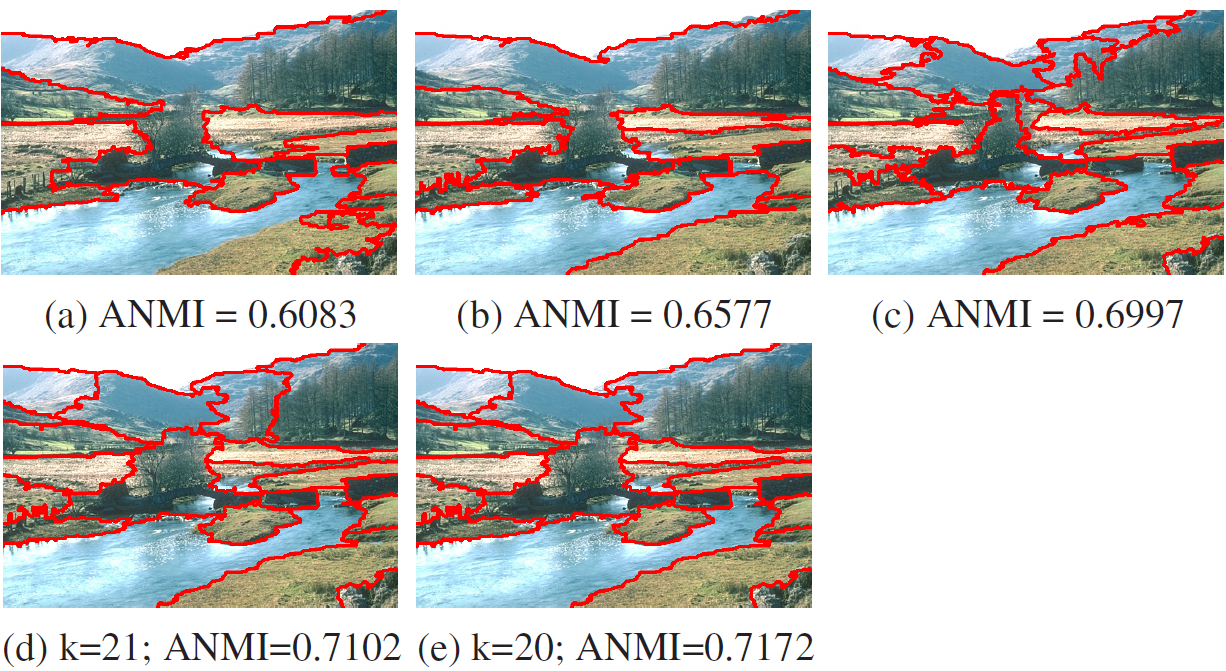
\includegraphics[width=0.7\linewidth,height=0.4\linewidth]{pic8}
	\end{figure}
(a)-(c) zeigen drei Eingabesegmentierungen mit
dem schlechtesten, dem mittleren und dem besten ANMI. (d)
Kombinierte Segmentierung mit dem vorgeschlagenen Algorithmus und
(e) Kombinierte Segmentierung mit optimalem K.
\end{frame}
\end{document}